\documentclass[fontsize=12pt]{article}
%\usepackage{xeCJK}
\usepackage{amsfonts}
\usepackage[makeroom]{cancel}
\usepackage{amssymb}
\usepackage{amsmath}
\usepackage{bm}
\usepackage{graphicx}
\usepackage{setspace}
\doublespacing
\newcommand{\td}{\cdot\cdot\cdot}
\newcommand{\cd}{\cdot}

\def\BibTeX{{\rm B\kern-.05em{\sc i\kern-.025em b}\kern-.08em
		T\kern-.167em\lower.7ex\hbox{E}\kern-.125emX}}

\newtheorem{theorem}{Theorem}[section]
\newtheorem{corollary}{Corollary}[theorem]
\newtheorem{lemma}[theorem]{Lemma}
\newtheorem{example}[theorem]{Example}
%\setCJKmainfont{SimSun}
\title{A Novel Method For Listing Low-Weight Parity Bit Codewords For Recursive Systematic Convolutional Codes} 
\author{Kwame Ackah Bohulu, Han Chenggao}
\date{\today}
\begin{document}
\maketitle

\newpage
\begin{abstract}
In this paper, we present a novel low-complexity method for listing input messages which produce codewords with low-weight parity bit sequences for  Recursive Systematic Convolutional Codes (RSCCs).
This method is implemented by  treating the RSCC as closed finite-state machine and determining all paths through the trellis that begin and end at state 0 for a given trellis length. Using the proposed method, we obtain a partial distance spectrum and calculate the upper-bound for the probability of bit error of the given RSC code. Simulation results reveal that the performance of the RSCC over the AWGN channel can be approximated using the codewords found by the proposed method.
\end{abstract}
	
\section{Introduction}

A Convolutional Code (CC) is generated by passing an input message through a linear finite-state shift register. The structure of this code is such that it is best described using a trellis. This structure makes it possible to employ soft decision decoding algorithms, the most popular of these algorithms being the Viterbi algorithm. CC are used extensively in mobile communication and space communication application as a major component in concatenated code.  Depending on the configuration of the shift register being used to generate the code, a CC can either be \textit{recursive} or \textit{nonrecursive}. In the case of the recursive CC, a feedback shift register is used to generate the code. Furthermore if the input message appears in the CC, it is known as \textit{systematic}. Recursive Sytematic Convolutional Codes(RSCC's) are used as component codes for Turbo codes, which are one of the few error correcting codes with performance very close to the Shannon limit [1].

Low weight codeword may be produced when the parity bit sequence has a very low weight. Amongst all such codewords, the one with the lowest weight determines the free distance $d_{\text{free}}$ of the code. 
$d_{\text{free}}$  of a RSCC is a very important factor and determines its error-correction performance [4].  This can be obtained from the distance spectrum of the RSCC which requires the calculation of the transfer function. %, where 
 As the number of states present in the RSCC increases so does the complexity involved in calculating the transfer function. Furthermore, the transfer function only provides information about the number of codewords of weight $d$ generated by an input message of weight $w$. There is no extra information with regards to the structure of the input message which generates which low-weight parity bit sequences and possibly low-weight codewords.

In this paper, we present a novel method which can be used to easily determine which input message of length $K$ will result in parity bit sequences which has a specific weight after it has been encoded with an RSC encoder. This method does not require the calculation of the transfer function of the RSCC. Using this method we calculate the theoretical upper bound for the given RSC code using the partial distance spectrum obtained. 

The rest of the research paper is organised as follows. In Section \ref{sec2}, we give a brief review of RSC codes. In section \ref{sec3}, we describe how the distance spectrum of a RSCC is obtained using the transfer function, followed by the presentation of our novel method in Section \ref{sec4}. Simulation results are presented in Section \ref{sec5} and we draw conclusions in Section \ref{sec6}


\section{Recursive Systematic Convolutional Codes:Review}
\label{sec2}

An $(n,k)$ RSCC is a convolutional code generated by using feedback shift registers which has its input bits as part of the codeword. At each time instant it receives an input of $k$ bits and outputs $n$ bits. The output bits are determined by the generator function, which may be written in $D$ notation as  $[1 ~\frac{F(D)}{B(D)}]$. Given the systematic nature of the RSCC, we only focus on the parity part of the RSCC and write the generator function simply as $[\frac{F(D)}{B(D)}]$ where $F(D)$ and $B(D)$ represent the feedfoward and feedback connections of the component encoder.  

It should be noted that the prescence of the feedback loop means that the code produced will have an infinite-length impulse response. A parameter which arises as a result of this infinite impulse response is know as the cycle length  [5], denoted by $\tau$, which is defined as the output cycle of an RSC encoder when the input is $[1 0 0 0 .....]$. We denote the impulse response of the RSCC by $\textbf{t}$.
 The cycle is represented by $\textbf{p}$ and is unique for each RSCC. 

\begin{figure}[h]
\centering
		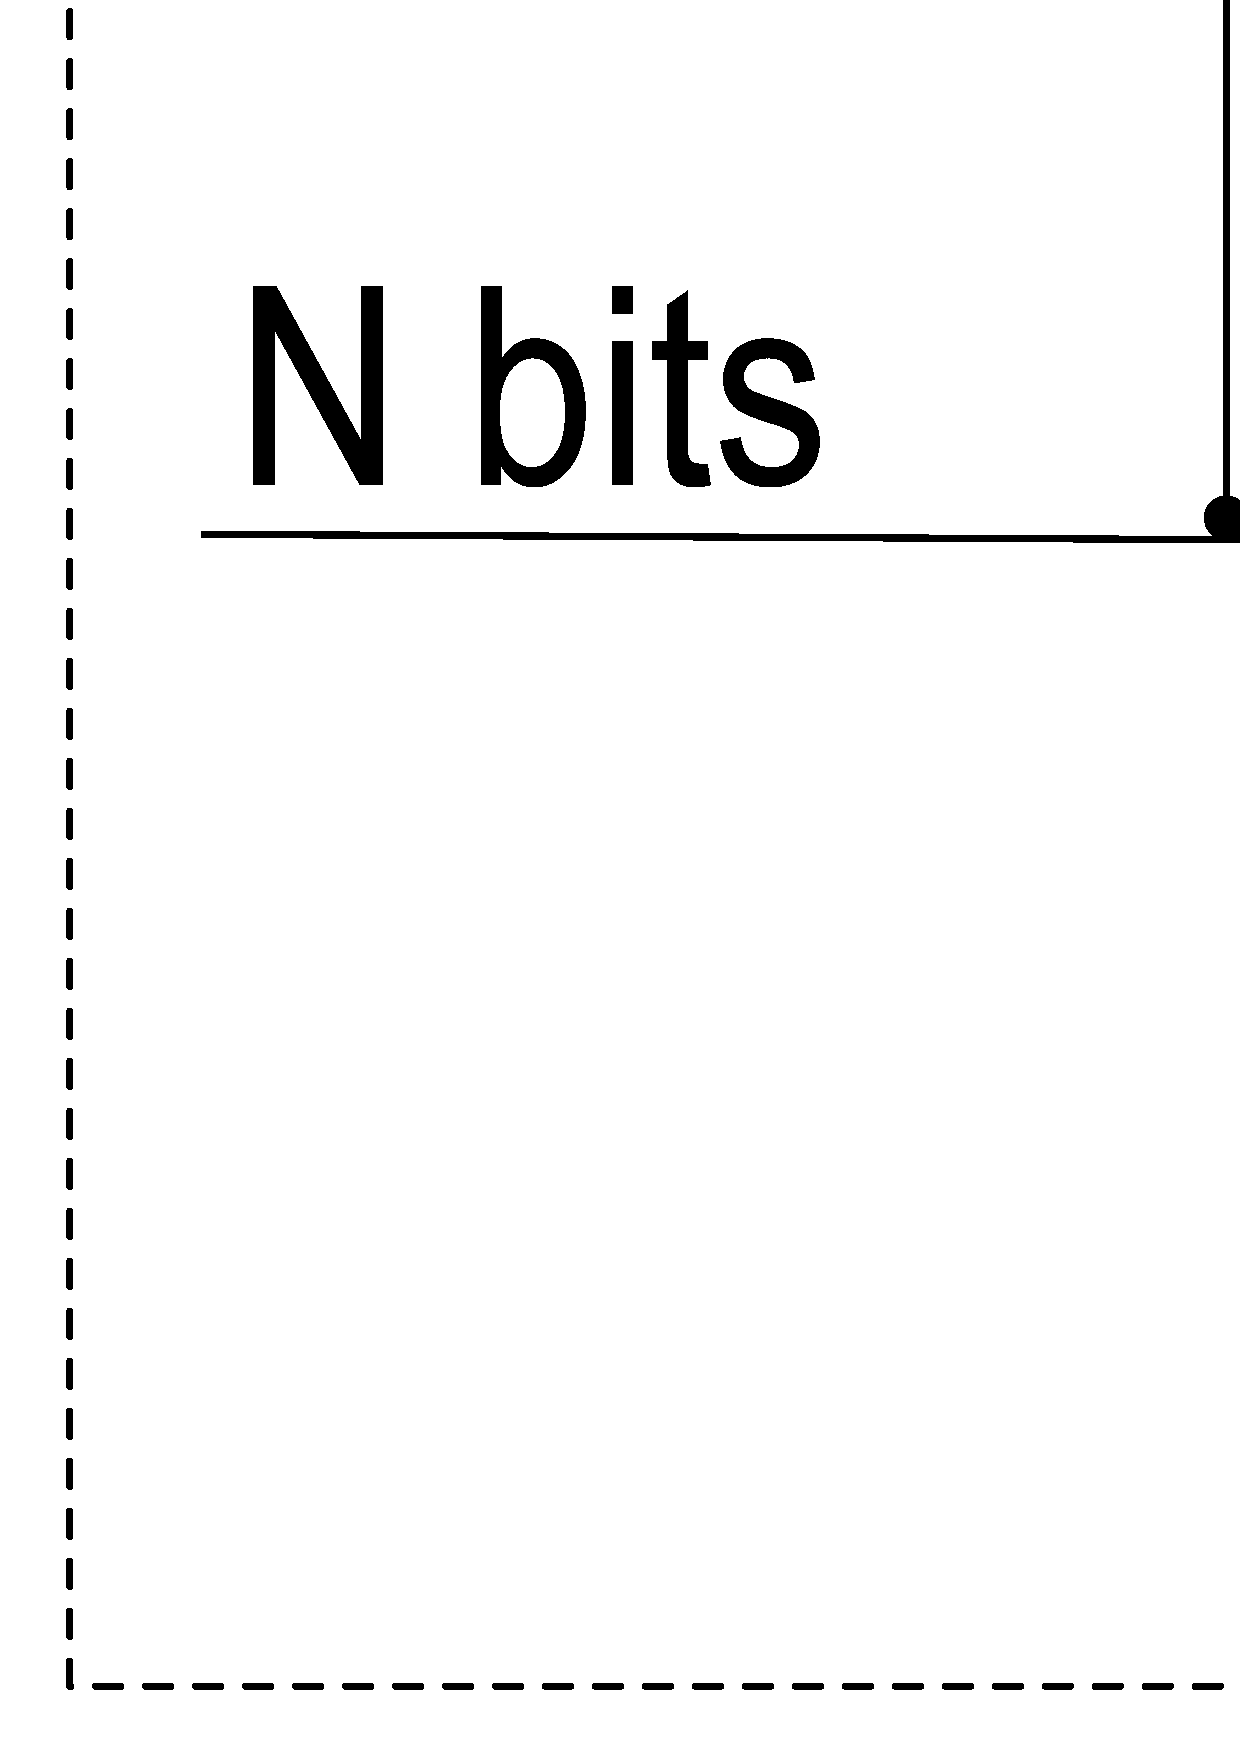
\includegraphics[width=0.45\textwidth]{RSCExample3.pdf}
		\caption{$[\frac{1+D^2}{1+D+D^2}]$  RSC Encoder}
		\label{fig1}
		\end{figure}
		
A RSC encoder is shown in Figure \ref{fig1}. Its generator function is given by $[\frac{1+D^2}{1+D+D^2}]$ which may be written as $5/7$ in octal form where $5 ~ \text{and} ~ 7$ correspond to the numerator and denomenator of the generator function respectively. 
 For the $5/7$ RSC code, the output is of the form $\textbf{t}=[1 1 1 0 1 1 0 1 1 0 ...]$ which gives us a cycle $\textbf{p}$ of $[1 1 0]$ and a cycle length $\tau =3$. Also $k=1$ and $n=2$. The knowledge of $\textbf{p}$ and $\tau$ will be used in deriving the method for determing which input messages generate low-weight parity bits. 
 
For the decoding of RSCC's, the Viterbi decoder is used. The idea is to go through the trellis of the RSCC and determine the most probable path through the trellis which corresponds to the transmitted input message.

\section{Transfer Function of RSCC}
\label{sec3}
The distance spectrum of code gives information about codeword weights and the number of such codewords present in the code. For the RSCC, this can be obtained from its transfer function denoted by $$T(Y,X)=\sum_{d=0}^{\infty}\sum_{w=0}^{\infty} a(d,w)Y^dX^w$$,  where $a(d,w)$ is the number of codewords of weight $d$ generated by an input message of weight $w$.
Based on the method described in [3], we outline the process involved in deriving the transfer function of the $5/7$ RSCC. 

\begin{figure}[h]
\centering
		\includegraphics[width=0.45\textwidth]{tf.png}
		\caption{State Diagram of the $5/7$ RSCC }
		\label{fig4}
		\end{figure}
First, the state diagram of the $5/7$ RSCC is redrawn as shown in Figure \ref{fig4}. The zero state is split into two and the transition from the zero state to itself is ommited. On each edge, the variables $Y^d$ and $X^w$ are used to represent the output weight $d$ and input weight $w$ of the path respectively. We treat each edge label as a transfer block and we employ the following rules for graph simplification. Assume two edge labels $H$ and $B$ 

   \begin{table*}[h]
 
 \caption{codewords with parity bit sequence weight $w_H(\textbf{h})=2$}
\centering
 \begin{tabular}{c c c c} 
 \hline
 $w_H(\textbf{b})$ & $a(x)$ & $b(x)$ & $h(x)$ \\ [0.5ex] 
 \hline\hline
 3 & 1 & $1+x+x^2$ & $1+x^2$\\ 
 4 & $1+x^2$ & $1+x+x^3+x^4$ & $1+x^4$ \\
 5 & $1+x^2+x^4$& $1+x+x^3+x^5+x^6$ & $1+x^6$ \\
 6 & $1+x^2+x^4+x^6$& $1+x+x^3+x^5+x^7+x^8$& $1+x^8$ \\
 7 & $1+x^2+x^4+x^6 +x^8$ & $1+x+x^3+x^5+x^7+x^9+x^{10}$ & $1+x^{10}$ \\
 8 & $1+x^2+x^4+x^6 +x^8 +x^{10}$ & $1+x+x^3+x^5+x^7+x^9+x^{11}+x^{12}$ & $1+x^{12}$\\ 
 9 & $1+x^2+x^4+x^6 +x^8+x^{10}+x^{12}$ & $1+x+x^3+x^5+x^7+x^9+x^{11}+x^{13}+x^{14}$ & $1+x^{14}$ \\ [1ex] 
 \hline
 \end{tabular}
 \label{tab1}
\end{table*}

\begin{enumerate}
\item If $H$ is connected in series to $B$, the labels are merged as $HB$

\item If $H$ is connected in parallel to $B$, the labels are merged as $H+B$

\item If the edges are in a feedback configuration, where $H$ and $B$ are the feedfoward and feedback portions respectively, the labels are merged as $\frac{H}{1-HB}$
\end{enumerate}

In the following, we demonstrate the process for deriving the transfer function for the RSCC shown in Figure {\ref{fig4}}. The respective state diagram transformations are also shown in Figure {\ref{fig5}}.

\begin{figure}[h!]
\centering
		\includegraphics[width=0.45\textwidth]{tfexample.png}
		\caption{State Diagram Transformations involved in Transfer Function Calculation }
		\label{fig5}
		\end{figure}

\begin{example} Define all edge labels\\
\label{ex3}
 edge $ a\triangleq 0 0 \rightarrow 1 0$,  edge $b \triangleq 1 0 \rightarrow 0 1$\\
 edge $ c \triangleq 0 1 \rightarrow 0 0$, edge $d \triangleq 0 1 \rightarrow 1 0$\\
 edge $ e \triangleq 1 0 \rightarrow 1 1$, edge $f \triangleq 1 1 \rightarrow 1 1$\\
 edge $ g \triangleq 1 1 \rightarrow 1 0$

\begin{enumerate}
\item Simplify edge $g$ with feedback configuration

$$ \frac{1}{1-YX}$$

\item Merge edges $e,f,g$ with series configuration and rename it edge $h$

$$\text{edge}~h = Y\times \frac{1}{1-YX}\times Y=\frac{Y^2}{1-YX}$$

\item Merge edges $h,b$ with parallel configuration and rename it edge $j$

$$\text{edge}~j = YX+ \frac{Y^2}{1-YX}= \frac{YX+Y^2X^2+Y^2}{1-YX}$$

\item Merge  edges $j,d$ with feedback configuration and rename it edge $k$ 
\begin{equation*}
\begin{split}
 \text{edge}~k&= \frac{\frac{YX+Y^2X^2+Y^2}{1-YX}}{1-(\frac{YX+Y^2X^2+Y^2}{1-YX})}\\
 &=\frac{Y(X-YX^2+Y)}{1-2YX+Y^2X^2-Y^2}
\end{split}
\end{equation*}

\item Calculate transfer function by merging edges $k,a,c$ with series configuration

\begin{equation*}
\begin{split}
T(Y,X)&=Y^2X \times \frac{Y(X-YX^2+Y)}{1-2YX+Y^2X^2-Y^2}\times Y^2X \\
&=\frac{Y^5X^2(Y-YX^2+Y)}{1-2YX+Y^2X^2-Y^2}\\
&=Y^5X^3+Y^6(X^4+X^2)+Y^7(X^5+3X^3)+\\
&Y^8(X^6+6X^4+X^2)+Y^9(X^7+10X^5+5X^3)+...
\end{split}
\end{equation*}
\end{enumerate}
\end{example}

From the example, it is clear that the complexity involved in deriving the transfer function increases as the number of states of the RSCC increases. Also to obtain the distance spectrum requires an extra division operation. Furthermore, with this method, it is impossible to get any extra detail regarding the structure of the input message bits which correspond to a codeword of a particular weight. We present a method which has less complexity and provides more information with regards to the distance spectrum in the next section.

\section{Method for Determining Parity Check Bit Weights}
\label{sec4}
As mentioned earlier, our interest is to determine if a given input message $\textbf{b}$ will produce low-weight parity bit sequence. In this section, we present a novel low-complexity method for determining such input messages. With the knowlege of the impulse response of the  RSC encoder and a little algebra, it is possible to determine what the parity bits will be and by extension, the weight of the parity bits. 

%$b(x) = b_0x^0+b_1x_1+...+b_{N-1}x_{N-1}$ 
Let $\textbf{b} =[b_0 b_1 ... b_{K-1}]$ be an input message of length $K$. We assume that $\textbf{b}$ is encoded using the $\frac{5}{7}$ RSC encoder to produce a codeword $\textbf{c}=[c_0 c_1 c_2 c_3 c_4 c_5 ... c_{M-1}]$, where $M=\frac{nK}{k}$. This codeword is formed from multiplexing  systematic bits and the parity bits. The systematic bits are made up of the input message itself and are found in the even numbered part of the codeword, whiles the parity bits are determined by the past and present input bits fed into the encoder. 
We represent the parity bits by 
$\textbf{h}=[h_0 h_1 h_2 ... h_{K-1}] \equiv [c_1 c_3 c_5 ... c_{M-1}]$

 We write $\textbf{b}$ and $\textbf{h}$ in polynomial form as $b(x)$ and $h(x)$. We also represent the impulse in polynomial form as $t(x)$. In the polynomial representation, only ``1'' bits are of interest. Also all calculations are carried out using modulo 2 arithmetic.
in general, $h(x)$ is calculated as (\ref{eq3})
 \begin{equation}
 \begin{split}
 h(x)&=t(x)b(x)\\
 \end{split}
 \label{eq3}
 \end{equation}
 
 (\ref{eq3}) can be intepreted as a convolution operation on $\textbf{t}$ by $\textbf{b}$. Figure \ref{fig6} shows two cases where a low-weight codeword might be generated. Within $\textbf{t}$ is a repitition of the cycle $\textbf{p}=[1 1 0]$. After the convolution operation, if the sum of the overlap is made up of $l$ cycles which overlap perfectly ( Figure \ref{fig6}(a)) or it is made up $j~\tau$ shifts of the cycle ( Figure \ref{fig6}(b)) , then the convolution sum of the overlap is $0$, where $l=\{2,4,6,...\}$ and $j=\{1,2,3,...\}$
 
 
 \begin{figure}[h]
\centering
		\includegraphics[width=0.35\textwidth]{overlap.png}
		\caption{Two cases where $\textbf{h}$ has low-weight parity bit sequence}
		\label{fig6}
		\end{figure}
		

 In other words, if $ h_p(x)=b(x)p(x)$ is a multiple of $1+ x^{\tau}$, then the convolution sum of the overlap will be $0$ and a low-weight codeword might be generated. $p(x)$ is the cycle $\textbf{p}$ of the  RSC code in polynomial form.
These cases are shown in Figure $\ref{fig6}$.
We may rewrite $ h_p(x)$ as
 \begin{equation}
 h_p(x)  \equiv b(x)p(x) ~\mod{ 1+ x^{\tau}}\\
 \label{eq1}
 \end{equation}

 
and if $h_p(x) = 0$, it mean that $b(x)$ generates a low weight parity bit sequence $h(x)$.  We may then write $b(x)$ as 
 $$b(x) \equiv  0 ~\mod{ g(x)} $$ which means it is possible to factorize $b(x)$ as 
 %$b(x) \equiv  0_{\tau}(x) ~\mod{ g(x)} $ 
 \begin{equation}
 b(x) =g(x)a(x)
 \label{eq2}
 \end{equation}
 where $a(x)$ is the quotient obtained after dividing $h_p(x)$ by $1+ x^{\tau}$
 
 Given $b(x)$ and $a(x)$, it is possible to calculate $g(x)$ via polynomial division.
 
 Fixing (\ref{eq2}) into (\ref{eq3}) we have 
 
 \begin{equation}
 \begin{split}
 h(x)&=t(x)b(x)\\
 &=t(x)g(x)a(x)\\
 & = o(x)a(x)
 \end{split}
 \label{eq4}
 \end{equation}
 where  $o(x)=t(x)g(x)$ and $o(x)$ is written ignoring all coefficients with order greater than $x^{\tau}$
 
 The process is explained further in Example  \ref{ex1}  and Example  \ref{ex1} for $\textbf{b}^{(0)}=[1 1 1]$ and  $\textbf{b}^{(1)}=[ 1 0 1]$ for the $5/7$ RSC encoder. The impulse response $t(x)=1+x+x^2+x^4+x^5+x^7+x^8+....~ \text{and}~p(x)=1+x$
 
 \begin{table*}[h!]
 
 \caption{codewords with parity bit sequence weight $w_H(\textbf{h})=4$}
\centering
 \begin{tabular}{c c c c} 
 \hline
 $w_H(\textbf{b})$ & $a(x)$ & $b(x)$ & $h(x)$ \\ [0.5ex] 
 \hline\hline
 2 & 1+x & $1+x^3$ & $1+x+x^2+x^4$\\ 
 \hline 
  & $1+x+x^2$& $1+x^2+x^4$& $1+x+x^3+x^4$ \\
   3 & $1+x+x^3$& $1+x^4+x^5$ & $1+x+x^2+x^5$ \\
  & $1+x^2+x^3$ & $1+x+x^5$ & $1+x^3+x^4+x^5$ \\
  \hline 
  & $1+x+x^2+x^3 $ & $1+x^2+x^3+x^5$ & $1+x+x^4+x^5$ \\
  & $1+x+x^2+x^4 $ & $1+x^2+x^5+x^6$ & $1+x+x^3+x^6$ \\
 4 & $1+x+x^3+x^5 $ & $1+x^4+x^6+x^7$ & $1+x+x^2+x^7$\\ 
  & $1+x^2+x^3+x^4 $ & $1+x+x^4+x^6$ & $1+x^{3}+x^5+x^6$ \\ 
  & $1+x^2+x^3+x^5 $ & $1+x+x^6+x^7$ & $1+x^{3}+x^4+x^7$ \\  
  & $1+x^2+x^4+x^5 $ & $1+x+x^3+x^7$ & $1+x^5+x^6+x^7$ \\ 
 [1ex]
 \hline
 \end{tabular}
 \label{tab2}
\end{table*}
  %In the case of the $5/7$ RSC code $\hat{i(x)}=1+x+x^2$ and therefore $h(x)=(1+x+ x^{2})(1+x+ x^{2}) = 1+x^2+ x^4 =1+x^2$ since everything from$ x^4$ is zero when $b(x) \equiv  0_{\tau}(x) ~\mod{ 1+x+ x^{2}} $

\begin{example}
\label{ex1}
$\textbf{b}^{(0)}=[1 1 1 ],~b^{(0)}(x)=1+x+x^2$

\begin{enumerate}
\item Determine if $h_p^{(0)}(x) =0$

\begin{equation*}
\begin{split}
h_p^{(0)}(x)& \equiv b^{(0)}(x)p(x) \mod{1+x^{\tau}}\\
& \equiv (1+x+x^2)(1+x)  \mod{1+x^{3}}\\
&\equiv 1+x^3  \mod{1+x^{3}} =0 ~\text{with remainder }~ a(x) =1
\end{split}
\end{equation*}

\item Find $g(x)$
 
 \begin{equation*}
 \begin{split}
 b^{(0)}(x)&=g(x)a(x) \\
 g(x) &=\frac{b^{(0)}(x)}{a(x)}\\
 &=\frac{1+x+x^2}{1}\\
 &=1+x+x^2
 \end{split}
 \end{equation*}
 
 \item Find $h^{(0)}(x)$
 \begin{equation*}
 \begin{split}
 h^{(0)}(x)&=t(x)g(x)a(x) \\
 &=(1+x+x^2+...)(1+x+x^2)(1)\\
 &=1+x^2  ~\text{and}~ o(x)=1+x^2 
 \end{split}
 \end{equation*}
 
\end{enumerate}
\end{example}

\begin{example}
\label{ex2}
$\textbf{b}^{(1)}=[1 0 1],~ b(x)=1+x^2$

\begin{enumerate}
\item Determine if $h_p^{(1)}(x) =0$

\begin{equation*}
\begin{split}
h_p^{(0)}(x)& \equiv b^{(1)}(x)p(x) \mod{1+x^{\tau}}\\
& \equiv (1+x^2)(1+x)  \mod{1+x^{3}}\\
&\equiv 1+x+x^2+x^3  \mod{1+x^{3}}\\ &=x+x^2 \neq 0
\end{split}
\end{equation*}
\end{enumerate}
\end{example}
 
 With this knowledge, it is possible to find the input message which produce low-weight parity bit sequences and by extension all codewords  with low-weight parity bits. Applying this method directly requires testing all message inputs of length $K$ which is time-consuming and very inefficeint. A better method will be to find all values of $a(x)$ which produce $h(x)$, where $h(x)$ has a low parity weight. This can be acheived using the finite state configuration shown in Figure \ref{fig2}, which is an application of (\ref{eq4}). The state table is shown in Table \ref{tab3}. 
 
\begin{figure}[h]
\centering
		\includegraphics[width=0.45\textwidth]{fsm.png}
		\caption{Finite State Machine Configuration}
		\label{fig2}
		\end{figure}
		
		
		
		The trellis length is set to $K$ and initial state is set to all-zero and the initial input into finite-state machine are set to $1$.  We trace all paths throught the trellis which begin and end at the all-zero state at a stage K of the trellis. $a(x)$ corresponds to the inputs which produce such paths and $b(x)$ corresponds to outputs produced by such paths. Once all valid paths are found we can calculate $g(x)$ using (\ref{eq4}) . Finally, we can find all corresponding values of $b(x)$ using (\ref{eq3}).
 
 For $K=16$ we find all $b(x) ~\text{and}~ c(x)$ for which $w_H(\textbf{c})=2 ~\text{and} ~ w_H(\textbf{c})=4$. The results are shown in Table \ref{tab1} and \ref{tab2} respectively . For $w_H(\textbf{c})=4$, only the first 10 results are shown. 
  For each stage in the trellis, the number of paths through the trellis is squared. To reduce the number of calculations per stage, we calculate the weight of the path and get rid of all paths that have an output weight greater than a target weight $w_H(\textbf{c})$
  \begin{table}[h!]
 
 \caption{State Table for Finite State Machine in Fig. \ref{fig2}}
\centering
 \begin{tabular}{c c c c} 
 \hline
 $a(x)$ & S & $S'$ & $h(x)$ \\ [0.5ex] 
 \hline\hline
 0 & $0 0 $& $0 0$ & $0$\\ 
  1& $0 0$ & $1 0$ & $1$ \\
  0 & $0 1$& $0 0$ & $1$ \\
  1& $0 1$& $1 0$& $0$ \\
  0& $1 0$ & $0 1$ & $0$ \\
 1 & $1 0 $ & $1 1$ & $1$\\ 
 0 & $1 1$ & $0 1$ & $1$ \\ 
 1 & $1 1$ & $1 1$ & $0$ \\ [1ex] 
 \hline
 \end{tabular}
 \label{tab3}
\end{table}
 
\section{Simulation Results}
\label{sec5}

In order to confirm the validity of the proposed method, we compared the bit error rate (BER) upper bound the RSCC to results obtained through computer simulations. 
%After an input message \textbf{b} is encoded, it is modulated using an appropriate modulation scheme and transmitted to the receiver over a channel. If the channel is AWGN, noise is added to the signal and the signal at the receiver is $\textbf{r}=[r_0,r_1,r_{2N-1}]$. The receiver demodulates the signal and uses appropriate decoding and detection schemes to produce an estimate of \textbf{b}, $\hat{ \textbf{b} }$. If a wrong decision is made, we say that an error has occurred. To measure how efficient a code is at correcting errors the Bit Error Rate (BER) is used. In most cases, the BER for a code not easily determined and bounds are calculated to give an idea as to how efficient the code is at correcting errors. 
There are a number of equations used to calculate the upper bound for the BER of a CC and these equations also apply to RSCC. For the case where the code is BPSK modulated and soft Viterbi decoding algorithm is used, the probability of bit error $P_b$ can be calculated using the equation below [3].

\begin{equation}
P_b \leq \frac{1}{k} \sum_{d=d_{\text{free}}}^{d_{\text{max}}} u(d) Q\Bigg( \sqrt{\frac{2dE_c}{N_0}}\Bigg)
\label{eq5}
\end{equation}
where $u(d)=\sum_{w=1}^{\infty} w~ a(d,w)$,  $E_c/N_0$ is the Signal to Noise ratio for the transmitted codeword, $d_{\text{max}}$ is the largest value of $d$ used in the estimation of $P_b$ and $d_{\text{free}}$ is the free distance of the code. This equation require the knowledge of the distance spectrum of the RSCC and using the method described in the previous section,we obtain the partial distance spectrum for all input messages $b(x)$ of length $K=64$ which produce low-weight parity bits
$h(x)$ where $w_H(\textbf{h})=2 ~\text{and} ~ w_H(\textbf{h})=4$.  We then use those terms with $d_{\text{max}}=8$ to calculate the probability of bit error using (\ref{eq5}). 

For the simulation results we set $K=64$ and use a $5/7$ RSC encoder with tail-biting structure to encode the input messages. The codeword are BPSK modulated and transmitted over the AWGN channel. The soft Viterbi algorithm is used for the decoding and detection operation.

\begin{figure}[h]
\centering
		\includegraphics[width=0.45\textwidth]{paperg2.png}
		\caption{Simulation and Upper Bounds for $5/7$ RSCC}
		\label{fig3}
		\end{figure}
		
		The simulation results are compared with the upper bound in Figure \ref{fig3}. 
	We deduce that it is possible to estimate the performance of the RSC code by the upper bound obtained using our novel method. The difference between the upper bound and the simulation results is $1.3730 \times 10^{-4}, 2.9960 \times 10^{-5},2.2800 \times 10^{-6}, 1.5668^{-7}$ for $E_b/N_0$ (dB) values of $4,5,6~\text{and}~7$ respectively. 
%We observe that for $E_b/N_o$ value of  $6$ dB, the upper bound is x dB away from the simulation results whiles it is y dB from the simulation results at an $E_b/N_o$ value of  $6$ dB

\section{Conclusion}
\label{sec6}

In this paper, we presented a method for listing input message which produce codewords with low-weight parity bit sequences for a for a given $(n,k)$ RSCC. Compared to the Transfer function method, it has low complexity and provides more information about distance spectrum of the RSCC. Using a specially configured finite state machine, we can obtain a partial distance spectrum which we use to calculate an upper bound for the RSCC.  





\begin{thebibliography}{99}
\bibitem{ref1}  C. Berrou, A. Glavieux and P. Thitimajshima, 
''Near Shannon limit error-correcting coding and
decoding: Turbo codes'', Proc. Intern. Conf. Communications (ICC), Geneva, 
Switzerland, pp. 1064-
1070, May 1993.
\bibitem{ref2} John G. Proakis, Masoud Salehi. ``Digital Communications'', 
Fifth Edition,Chapter 8, McGraw-Hill.
\bibitem{ref3} Todd K. Moon. ``Error Correcting Codes'',Chapter 12, John Wiley \& Sons.
\bibitem{ref4}Alain Glavieux, ``Channel Coding in Communication Networks'',\\ Chapter 3, John Wiley \& Son. 

\bibitem{ref5} Jing Sun, Oscar Y. Takeshita ''Interleavers for Turbo Codes Using 
Permutation Polynomials over Integer Rings'', IEEE Trans. Inform. Theory, vol. 51, 
pp. 101 - 119  Jan. 2005.

\end{thebibliography}
\end{document}